\documentclass[12pt]{article} 

\usepackage{amsmath,amssymb,amsfonts}
\usepackage{psfrag}
\usepackage{color}
\definecolor{darkblue}{rgb}{0.1,0.1,.7}
\usepackage[colorlinks, linkcolor=darkblue, citecolor=darkblue, urlcolor=darkblue, linktocpage]{hyperref} 
\usepackage[square, comma, compress,numbers]{natbib}
\usepackage[]{amsmath}
\usepackage[]{graphicx}
\usepackage[]{latexsym}
\usepackage{geometry}
\usepackage{amscd}
\usepackage[all,cmtip]{xy}
\usepackage{mathrsfs}
\usepackage[margin=10pt,font=small,labelfont=bf]{caption}
\geometry{verbose,letterpaper,tmargin=2.5cm,bmargin=2.5cm,lmargin=2.6cm,rmargin=2.6cm}
\usepackage{dsdshorthand}
\usepackage{changepage}
\usepackage{listings}
\setlength{\parskip}{0.1in}
\hyphenpenalty=1000

\numberwithin{equation}{section}

\renewcommand{\be}{\begin{eqnarray}}
\renewcommand{\ee}{\end{eqnarray}}
\newcommand\nn{\nonumber}
\newcommand\cS{\mathcal{S}}
\newcommand\cR{\mathcal{R}}
\newcommand\SDPAGMP{\texttt{SDPA-GMP}}
\newcommand\SDPB{\texttt{SDPB}}
\newcommand\repl[1]{$\langle$\textrm{\em #1}$\rangle$}
\newcommand\defn[1]{\textrm{\em #1}\ $\equiv$}


\begin{document}

{\Large
\begin{center}
{\bf Outer Limits \\\vspace{.1in}}
\end{center}
}
\begin{center}
\noindent \today
\end{center}
\tableofcontents
\section{Introduction}
\label{sec:introduction}

\texttt{Outer\_Limits} is an experimental arbitrary-precision
semidefinite program solver, much like \texttt{SDPB}, but with a
markedly different strategy.  \texttt{SDPB} will find a solution by
adding up polynomial matrices which are each guaranteed to be
semidefinite.  This sum becomes more and more ill-conditioned matrix
as \texttt{SDPB} iterates towards a solution.  This ill-conditioned
matrix must be inverted in order to continue to the next iteration,
causing numerical problems.  \texttt{SDPB} overcomes this by requiring
very large precision arithmetic.

\texttt{Outer\_Limits}, on the other hand, starts by enforcing positive
semidefiniteness only at a finite set of points.  These are constant
constraints, so there is no longer a problem with ill-conditioned
matrices.  This allows \texttt{Outer\_Limits} to find a solution using
much lower precision.

Initially, this will find a solution that is, in general, not positive
semidefinite everywhere.  So \texttt{Outer\_Limits} will add more
points to the places where the function is not positive semidefinite
and find another solution.  This iterative procedure continues until
the solution is positive everywhere.

This strategy also allows \texttt{Outer\_Limits} to be more easily
applied to general problems.  \texttt{SDPB} requires that all inputs
be approximated as polynomials.  \texttt{Outer\_Limits}, in contrast,
only requires evaluations of the functions at zeros of Chebyshev
polynomials.

\texttt{Outer\_Limits} is bundled with \texttt{SDPB}.  See
\texttt{Install.md} for up-to-date instructions on getting pre-made
binaries or building from source.

\section{Semidefinite Problems}
\label{sec:semidefinite}

Consider a system with $J$ blocks.  Within each block, there is a set
of inequality constraints on an $N$-dimensional vector $y$.  In
addition, there is a known vector $b$, independent of the blocks.  The
goal of semidefinite programming is to find a solution to these
constraints while trying to maximize the quantity $b\cdot y$.

Writing this more formally, consider a collection of symmetric $R_{j}\times R_{j}$ matrices
\begin{eqnarray}
\label{eq:sdp}
M_j^n(\Delta) &=& \begin{pmatrix}
m_{j,11}^{n}(\Delta) & \dots & m_{j,1m_j}^{n}(\Delta)\\
\vdots & \ddots & \vdots\\
m_{j,R_j1}^{n}(\Delta) & \dots & m^{n}_{j,R_jR_j}(\Delta)
\end{pmatrix}
\end{eqnarray}
where $0 \leq n \leq N$ and $1 \leq j \leq J$, and each element
$m_{j,rs}^{n}(\Delta)$ is an arbitrary function in $\Delta$.  Define
the matrix $F_j\left(\Delta\right)$
\begin{equation}
F_j\left(\Delta\right)=M^0_j(\Delta)+\sum_{n=1}^{N} y_n M^n_j(\Delta).
\end{equation}
Then given $b\in \R^N$, \texttt{Outer\_Limits} will solve for coefficients $y_n$
that
\begin{eqnarray}
\label{eq:SDPconstraints}
\begin{array}{ll}
\textrm{maximize} & b_0+b\.y\quad\textrm{over}\quad y \in \R^N,\\
\textrm{such that} & F_j\left(\Delta\right) \succeq 0 \quad \textrm{for all $\Delta\geq 0$ and $1 \leq j \leq J$}.
\end{array}
\end{eqnarray}
The notation $F_j\left(\Delta\right)\succeq 0$ means $F_j\left(\Delta\right)$ is positive semidefinite.

\section{Input}
\label{sec:input}

Since \texttt{Outer\_Limits} solves these problems on a computer,
there are inevitable approximations that must occur.  The main one is
that the functions $m_{j,rs}^{n}(\Delta)$ must be well approximated by
a series of Chebyshev polynomials.  Specifically, the input to
\texttt{Outer\_Limits} is not the functions $m_{j,rs}^{n}(\Delta)$,
but rather their values at Chebyshev zeros and their relative sizes
near zero and at infinity.

The example in the \texttt{SDPB} Manual is
\begin{eqnarray}
  f_1 & = & 1 + \Delta^4, \\
  f_2 & = & \Delta^2 + \frac{\Delta^4}{12}.
\end{eqnarray}
This is a system with a single block ($J=1$) and two weights ($N=2$).
We will approximate these functions by Chebyshev polynomials covering
$0$ to $\Delta_{j,max}$.  So we need to decide on a $\Delta_{j,max}$
that is sufficient to cover all of the places where the functions
might go to zero.  In general, we want to choose a large enough
$\Delta_{j,max}$ such that the functions are dominated by the largest
terms at infinity.  In this case, the functions $f_1$ and $f_2$ have
polynomial terms that are of equal size at $\Delta=1$ and
$\Delta=\sqrt{12}\simeq 3.464$ respectively.  So to be conservative,
we choose $\Delta_{j,max}=100$.  Currently, \texttt{Outer\_Limits}
requires $\Delta_{j,max}$ to be the same for each function in a block.

Now we need to evaluate $f_1$ and $f_2$ at scaled and translated zeros
of Chebyshev polynomials.  This means that for an approximation with
$N$ points, we need values at
\begin{eqnarray}
\Delta_{j,k} =  \frac{\Delta_{j,max}}{2} \left(1 + \cos\left({\frac{\pi \left( k + \frac{1}{2} \right)}{N}}\right)\right), \textrm{ } 0 \le k < N
\end{eqnarray}
Since $f_1$ and $f_2$ are polynomials, we could use $N=5$ to get a
perfect approximation.  For this exercise, we will pretend we do not
know that and choose $N=10$.  \texttt{Outer\_Limits}
currently requires $N$ to be the same for each function in a block.

After generating the value of these functions at these points, we must
characterize the relative behavior of the different functions near
zero and at infinity.  This characterization turns out to be important
for computing high precision answers for the objective.

In this case, the characterization is straightforward.  $f_1$ and
$f_2$ are both degree=4 polynomials.  Near zero, $f_1$ goes to a
constant term and $f_2$ goes to zero.  So we can use $f_{1}(0)=1$ and
$f_{2}(0)=0$ for the limiting behavior near zero.  If $f_1$ did not
have a constant term, then we would have to compare the relative sizes
of the lowest degree non-zero coefficient.  At infinity, we only need
to know the relative sizes of the coefficients of $\Delta^4$: $1$ and
$1/12 \sim 0.083333333333333$.

Now we can construct the \texttt{functions} input file shown in
listing~\ref{lst:functions}.

\begin{lstlisting}[
  caption={\texttt{functions} input file.  The first block is $f_1$, and the second block is $f_2$.},
  label=lst:functions,
  mathescape,
  columns=fullflexible,
  frame=single,
  escapeinside=@@,
  basicstyle=\small\ttfamily\selectfont,
]
{
 "objective": ["0", "-1"],
 "normalization": ["1", "0"],
 "functions":
 [
  [
   [
    [
     {
      "max_delta" : "100",
      "epsilon_value" : "1",
      "infinity_value" : "1",
      "chebyshev_values" :
      [
       "1.1435973374045645814919250171",
       "883.02729988511593507402953969",
       "45996.705504467834968336421068",
       "555496.84436116128227452603002",
       "3164867.0107610102130932508775",
       "11178001.455036876356972361751",
       "27933561.314132283966434754990",
       "53079005.294495532165031663578",
       "79919384.706784958935035978021",
       "97560312.498026486725689472807"
      ]
     },
     {
      "max_delta" : "100",
      "epsilon_value" : "0",
      "infinity_value" : "0.08333333333333333333333333333333333333333",
      "chebyshev_values" :
      [
       "0.3909088380370479104722553418",
       "103.20121941417842758517038120",
       "4047.4415527729152920238132784",
       "47036.636299366781486947578226",
       "265517.84125951408811424149736",
       "934843.38959957190879426845671",
       "2333081.9137776891397492374085",
       "4430535.8917805604180413095200",
       "6668888.4064183873419762575987",
       "8139903.2205172185244035518177"
      ]
     }
    ]
   ]
  ]
 ]
}
\end{lstlisting}

The exact format is specified in the JSON schema
\texttt{docs/functions\_schema.json}.  At its heart, there is a set of
nested arrays.  The outermost array corresponds to the $j$ index of
$m_{j,rs}^{n}(\Delta)$, followed by $r$, $s$, and $n$.  The toy
example has $N=2$, $J=1$, and $R_{1}=1$, so $j=r=s=1$ and $n=1$ or
$2$.

The last thing to do is to create a \texttt{points} file that contains
the values of $\Delta$ where \texttt{Outer\_Limits} will initially
apply positivity constraints.  \texttt{Outer\_Limits} will also apply
constraints at epsilon and infinity.  At a minimum, you will need to supply enough
points such that there are at least as many constraints as there are
degrees of freedom in $y$.

For the toy problem, there are only two functions, so in principle you
only need two points.  Epsilon and infinity are always used, so you
not add any more points.  In practice, \texttt{Outer\_Limits} will get stuck if
you do not exceed the minimum by a healthy margin.

With that in mind, we choose the two points, $0.1$ and $1$,
resulting in the \texttt{points} input file in listing \ref{lst:points}.
Needless to say, the choice of points will depend strongly on the
problem you are solving.

\begin{lstlisting}[
  caption={\texttt{poinst} input file},
  label=lst:points,
  mathescape,
  columns=fullflexible,
  frame=single,
  escapeinside=@@,
  basicstyle=\small\ttfamily\selectfont,
]
{
 "points": [["0.1", "1"]]
}
\end{lstlisting}

The format for this file is specified in the JSON schema
\texttt{docs/points\_schema.json}.  The outer array corresponds to the
$j$ index of $m_{j,rs}^{n}(\Delta)$, and the inner array is a list
of points for that index.

\section{Running \texttt{Outer\_Limits}}
\label{sec:running}

\subsection{Initial Iteration and Scaling}
\label{subsec:initial}

When \texttt{Outer\_Limits} is running, it will first try to solve
equation \ref{eq:SDPconstraints}, but with a duality gap of 1.1.  This
very relaxed constraint on the duality gap allows it to quickly get a
very approximate solution.  Also, \texttt{Outer\_Limits} is only
enforcing the solution at the initial points via constant constraints.

One wrinkle here is that \texttt{Outer\_Limits} applies several
transformations in order to scale the problem before making use of
\texttt{SDPB}.  In the usual formulation, \texttt{SDPB} maximizes
\begin{eqnarray}
  b\cdot y
\end{eqnarray}
subject to the constraints
\begin{eqnarray}
  Y + B\cdot y & = & c\\
  Y \succeq 0
\end{eqnarray}
$B$ is a matrix corresponding to $M^n_j$, and $c$ is $M^0_j$, both evaluated
at the initial values of $\Delta$.  However, the relative sizes
of $c$ and the columns of $B$ can be wildly different, leading to
numerical difficulties.  To ameliorate this, we first find $c_{\max}$,
the largest value of $|c|$.  If $c$ is completely zero, we use
$c_{\max}=1$.

Next, we compute the singular value decomposition of $B$
\begin{eqnarray}
  B = U \Sigma V^T.
\end{eqnarray}
$U$ and $V$ are real orthogonal matrices, and $\Sigma$ is a rectangular
diagonal matrix with non-negative entries.  We define new
variables
\begin{eqnarray}
  y' & = & \Sigma V^T y/c_{\max}\\
  b' & = & b V \Sigma^{\dagger}c_{\max}\\
  c' & = & c/c_{\max}\\
  Y' & = & Y/c_{\max}\\
  B' & = & B V \Sigma^{\dagger}/c_{\max}
           \label{eq:Bprime}
\end{eqnarray}
where $\Sigma^{\dagger}$ is the pseudo-inverse of $\Sigma$.  In this
case, $\Sigma^{\dagger}$ is the transpose of $\Sigma$ with the
diagonal entries inverted.  So $\Sigma^{\dagger}$ is easy to compute
once we have $\Sigma$.  The system that we initially solve with
\texttt{SDPB} routines is then
\begin{eqnarray}
  \textrm{maximize}~b'\cdot y'
\end{eqnarray}
subject to the constraints
\begin{eqnarray}
  Y' + B'\cdot y' & = & c\\
  Y' \succeq 0
\end{eqnarray}

Computing the singular value decomposition of $B$ is relatively
expensive, similar in cost to completing a single iteration of
\texttt{SDPB}.  To amortize this cost over the whole calculation, we
save the expression $V \Sigma^{\dagger}$.  Then, at each iteration, we
compute a new $B'$ using equation \ref{eq:Bprime}.  With this method,
$B'$ is only guaranteed to be unitary on the first iteration.
However, later iterations will only add rows to $B$, so it should
still work reasonably well at equalizing the columns.

\subsection{Adapted Mesh}
\label{subsec:adaptedmesh}

With an initial solution in hand, the next step is to check for
regions within each block where the functional is negative.  To enable
this, \texttt{Outer\_Limits} creates a coarse mesh of
cells over the range from $0$ to $\Delta_{j,max}$.  Within each cell,
it evaluates the functional $F_j$ using the Chebyshev approximations
for $M_j^n$ and the solution values for $y_n$.  If the functional has
too much curvature and the points are not so close together as to
cause numerical difficulties, it splits the cell into smaller cells.

To be precise, for each block, we compute the largest value of the
functional among all the Chebyshev zeros
\begin{eqnarray}
  F_{j,\max} = \max \left( \left| F_{j} \left(\Delta_{j,k} \right) \right| \right)
\end{eqnarray}
In addition, for a cell with a width $\delta$, we define an interpolated averaged value
\begin{equation}
  \overline{F}_j\left(\Delta\right) = \left( F_j\left(\Delta + \delta\right) + F_j\left(\Delta - \delta\right) \right) /2
\end{equation}
Then we split the cell if the interpolated averaged value differs too
much from the actual value at that point
\begin{eqnarray}
  \left|\overline{F}_j\left(\Delta\right) - F_j\left(\Delta\right)\right| & < & \epsilon_{\rm{relative}} \left|\overline{F}_j\left(\Delta\right) + F_j\left(\Delta\right)\right| /2\\
  \left|\overline{F}_j\left(\Delta\right) - F_j\left(\Delta\right)\right| & < & \epsilon_{\rm{absolute}} F_{j,\max}.
\end{eqnarray}
The tolerance $\epsilon_{\rm{relative}}=\frac{1}{64}$ is somewhat
arbitrary.  The goal is to catch all of the places where $F_j$ varies
strongly, and in this way we can find all of the places where it
becomes negative.

The tolerance $\epsilon_{\rm{absolute}}$ is the smallest difference from 1
that can be represented, given the working precision.  For example,
with IEEE 754 double precision floating point numbers, this is
2.22045e-16.

\subsection{Checking Positivity}
\label{subsec:checkingpositivity}

With this adapted mesh in place, \texttt{Outer\_Limits} checks every
cell for positivity. For each cell, we compute the first and
second derivative numerically
\begin{eqnarray}
  dF_{j} & = &\left( F_{j}\left( \Delta + \delta \right) - F\left( \Delta - \delta \right) \right)/\left( 2 \delta \right),\\
  d^{2}F_{j} & = & \left( F_{j}\left( \Delta + \delta \right) - 2 F\left( \Delta \right) + F\left( \Delta - \delta \right) \right)/ \delta^2.
\end{eqnarray}
Using these to form a quadratic approximation to $F_{j}$, we compute
the location and value where $F_{j}$ is minimum
\begin{eqnarray}
  \Delta_{\min} & = & \Delta - dF_{j}/d^{2}F_{j},\\
  F_{\min} & = & F\left(\Delta\right) - \left(dF_{j}\right)^{2} /\left( 2 d^{2}F_{j}\right).
\end{eqnarray}

At first, we might think that only if $F_{\min}<0$ do we need to add
$\Delta_{\min}$ to the list of constraint points.  However, if
$F_{\min}>0$, it may only be positive due to inaccuracies in the
quadratic approximation.  Conversely, if $F_{\min}<0$, it may only be
negative due to inaccuracies in the finite precision arithmetic.  To
handle these cases, we add $\Delta_{\min}$ to the list of constraint
points if and only if
\begin{eqnarray}
  F_{\min} & < & \left| F\left(\Delta\right) - \overline{F}_j\left(\Delta\right) \right|, \\
  \left|F_{\min}\right| & > & \epsilon_{\rm{absolute}}F_{j,\max}.
\end{eqnarray}

\subsection{Further Iterations and Termination Criteria}
\label{subsec:furtheriterations}

With these new points, \texttt{Outer\_Limits} creates and solves a new
system as in section \ref{subsec:initial}.  Eventually, there will be
no new points.  Then \texttt{Outer\_Limits} reduces the duality gap by
\texttt{dualityGapReduction} and iterates again until there are no new
points.  \texttt{Outer\_Limits} continues this cycle of finding new
points and reducing the duality gap until the duality gap is less than
\texttt{dualityGapThreshold}.  This guarantees that the final result
will fully satisfy all of the constraints in \ref{eq:SDPconstraints}
without having to spend a lot of effort computing highly precise
solutions for very approximate problems.

\section{Output of \SDPB}

\subsection{Terminal Output}

The output from running \texttt{Outer\_Limits} on the example problem
in section \ref{sec:input} is in listing
\ref{listing:exampleoutput}. The beginning is very similar to
\texttt{SDPB}.  When iterating, \texttt{Outer\_Limits} first prints
the current number of constraints, including all of the blocks, and
the current gap threshold.  After each iteration,
\texttt{Outer\_Limits} prints the full array of weights and the
computed value of the objective.  If \texttt{Outer\_Limits} decides
not to add points, it will reduce the duality gap threshold, print
this new threshold, and continue with the current solution.

Figures \ref{fig:plot1}, \ref{fig:plot2}, and
\ref{fig:plot3} show the behavior of $F_0$ during the iterations
as it alternates between adding points and reducing the gap threshold.

\begin{lstlisting}[
  caption={Output of \texttt{Outer\_Limits} for the input file in listing~\ref{lst:points}},
  columns=fullflexible,
  label=listing:exampleoutput,
  keepspaces=true,
  basicstyle=\scriptsize\ttfamily\selectfont,
]
Outer_Limits started at 2021-Jun-16 21:16:54
functions file  : "test/toy_functions.json"
out directory   : "test/toy_functions_out.json"

Parameters:
dualityGapReduction          = 1024
maxIterations                = 1000
maxRuntime                   = 9223372036854775807
checkpointInterval           = 3600
findPrimalFeasible           = false
findDualFeasible             = false
detectPrimalFeasibleJump     = false
detectDualFeasibleJump       = false
precision(actual)            = 128(128)
dualityGapThreshold          = 1e-10
primalErrorThreshold         = 1e-10
dualErrorThreshold           = 1e-10
initialMatrixScalePrimal     = 10
initialMatrixScaleDual       = 10
feasibleCenteringParameter   = 0.1
infeasibleCenteringParameter = 0.3
stepLengthReduction          = 0.7
maxComplementarity           = 1e+100
initialCheckpointDir         = "test/toy_functions.ck"
checkpointDir                = "test/toy_functions.ck"
writeSolution                = 
verbosity                    = 1

num_constraints: 4
Threshold: 1.1
weight: [1, 17.9200220901249930755098639008252582465]
optimal: -17.9200220901249930755098639008252582465
Threshold: 0.001074218750000000086736173798840354720596
weight: [1, -1.845764788512892377453602431656624264456]
optimal: 1.845764788512892377453602431656624264454
Saving checkpoint to    : "test/toy_functions.ck"
num_constraints: 5
Threshold: 0.001074218750000000086736173798840354720596
weight: [1, -1.839611388308253894657545680555773464748]
optimal: 1.839611388308253894657545680555773464748
Threshold: 1.049041748046875084703294725430033906832e-06
weight: [1, -1.840275804402260393066356407589470103775]
optimal: 1.840275804402260393066356407589470103773
Saving checkpoint to    : "test/toy_functions.ck"
num_constraints: 6
Threshold: 1.049041748046875084703294725430033906832e-06
weight: [1, -1.840265160571370863263682954232296794857]
optimal: 1.840265160571370863263682954232296794854
Threshold: 1.024454832077026449905561255302767487141e-09
weight: [1, -1.840265762727976760495004292302021649703]
optimal: 1.840265762727976760495004292302021649702
Threshold: 1e-10
weight: [1, -1.840265763127732853472949500621348513756]
optimal: 1.840265763127732853472949500621348513754
Saving checkpoint to    : "test/toy_functions.ck"
optimal: 1.840265763127732853472949500621348513754
Saving solution to "test/toy_functions_out.json"
\end{lstlisting}

\pagebreak

\begin{figure}
\begin{center}
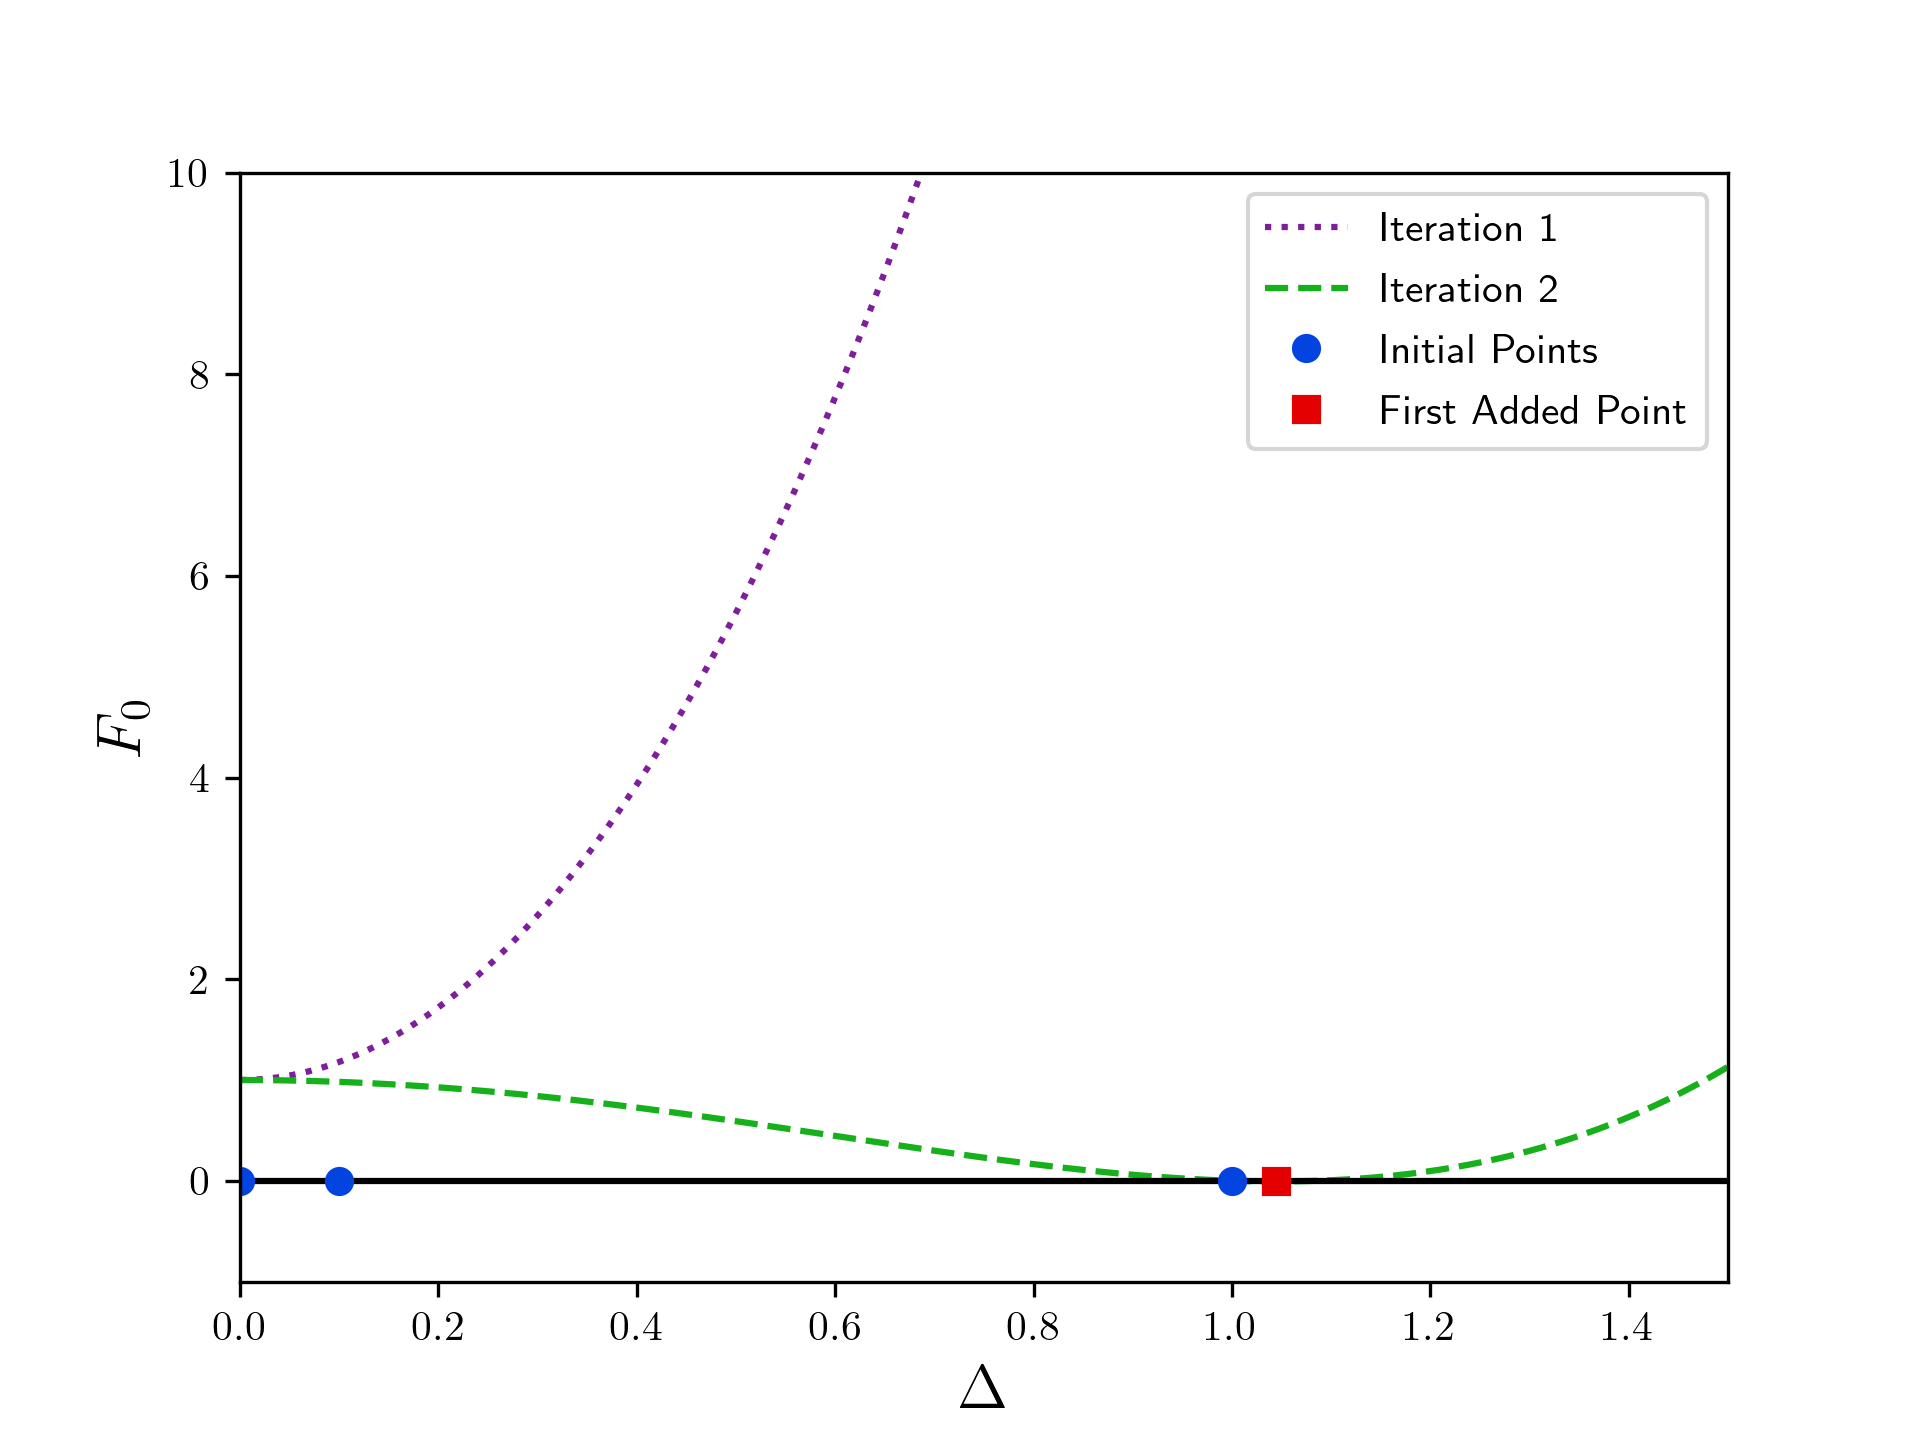
\includegraphics[width=0.9\textwidth]{outer_plots_1}
\end{center}
\caption{Plot of $F_{0}=y_{0}\left(1+x^4\right) + y_{1}\left(\frac{x^4}{12} + x^2\right)$
  after the first iteration, with duality gap threshold=1.1, and the second
  iteration, with duality gap threshold=$1.07\times10^{-3}$.  After the second
  iteration, \texttt{Outer\_Limits} adds a point at 1.044.}
\label{fig:plot1}
\end{figure}

\begin{figure}
\begin{center}
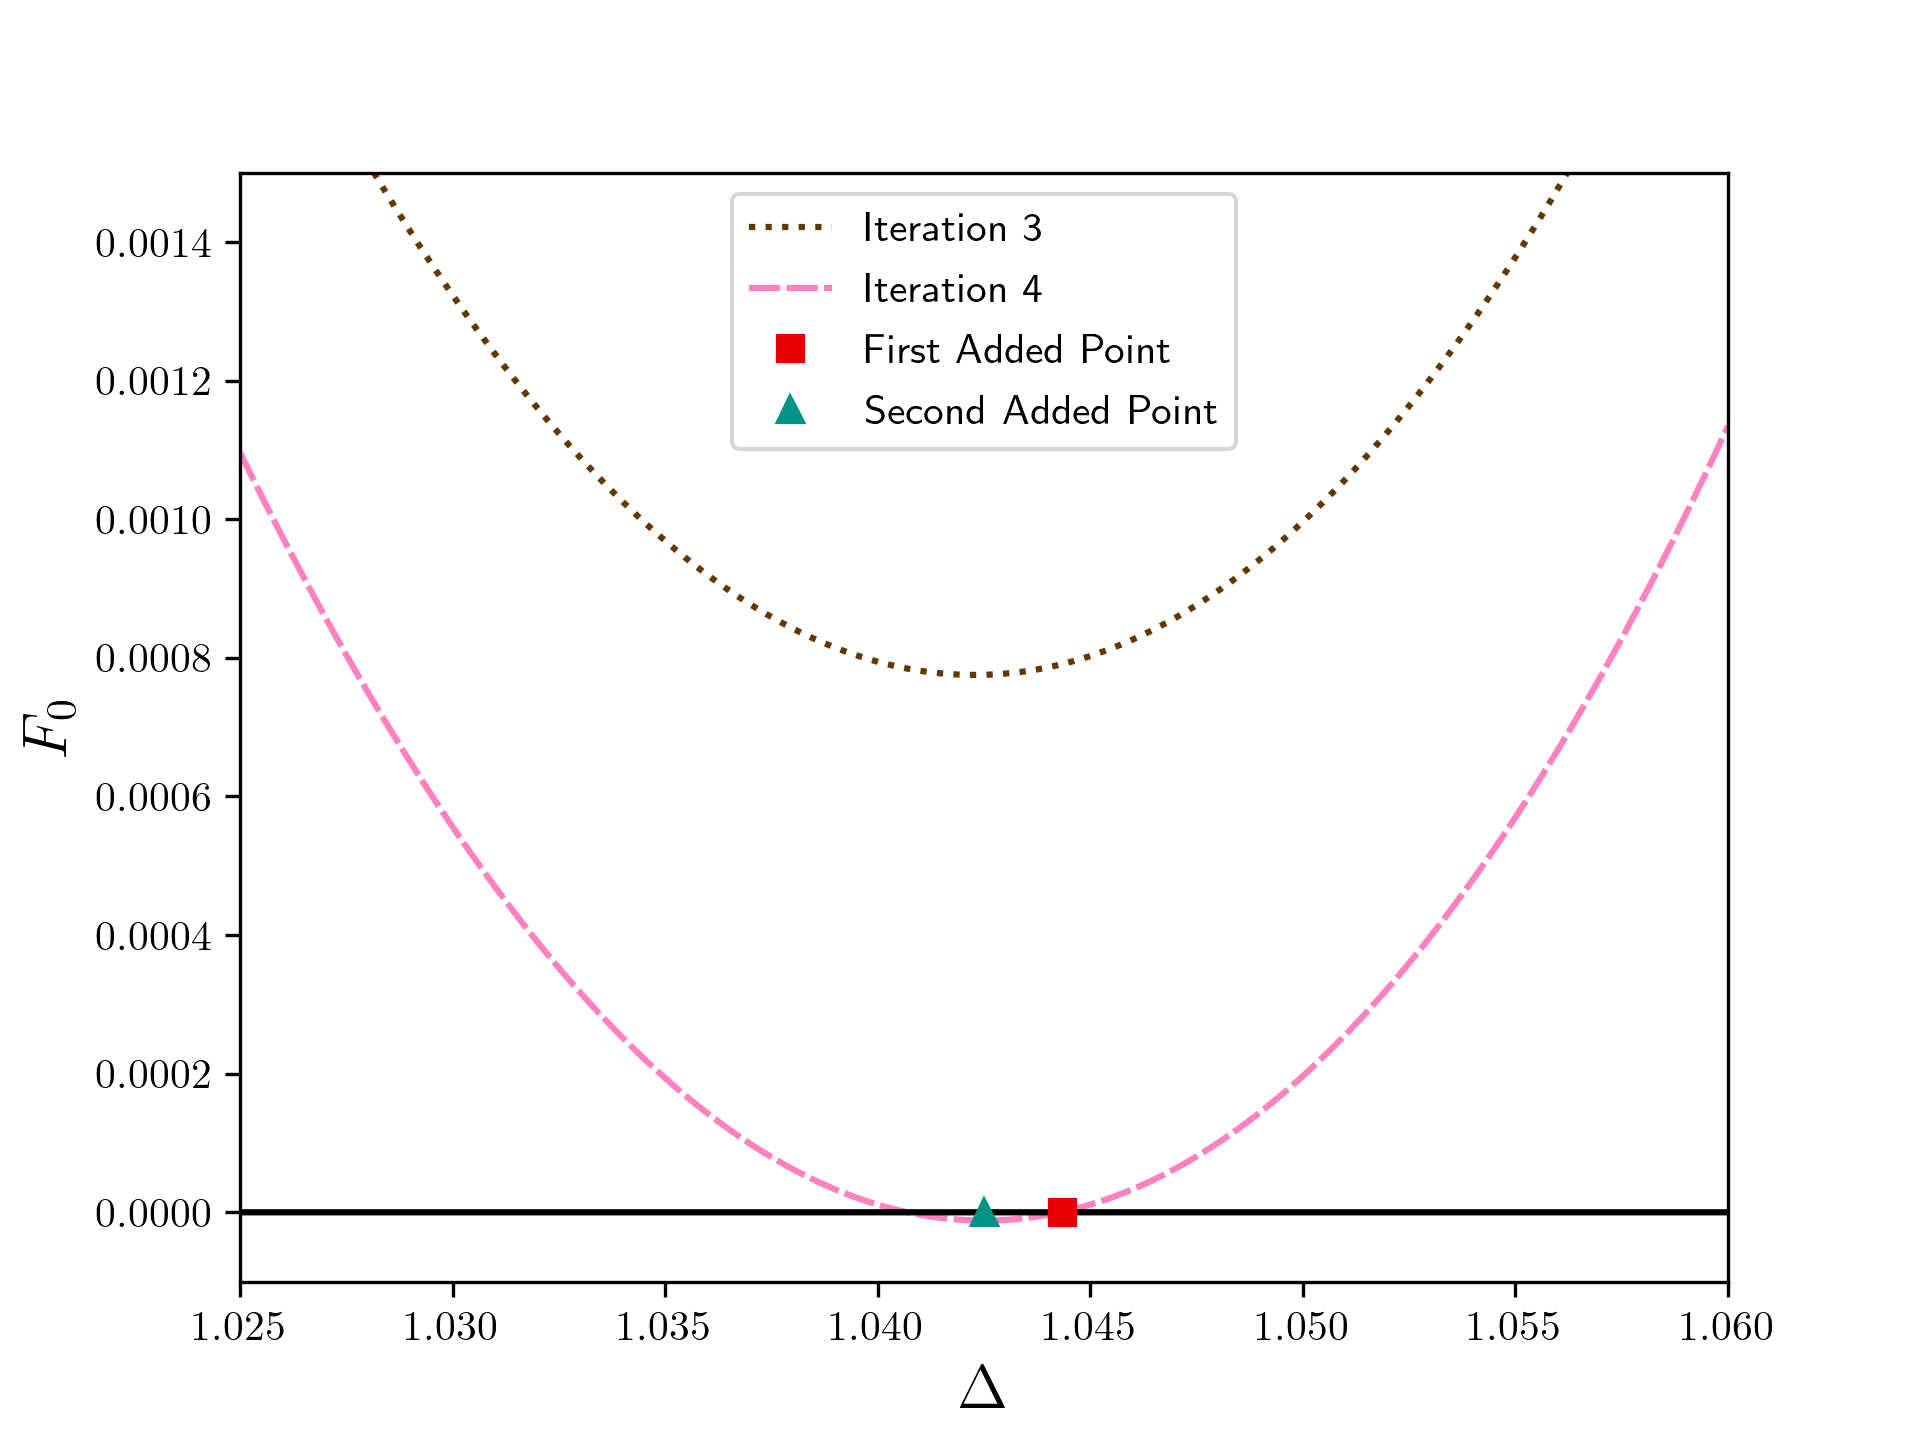
\includegraphics[width=0.9\textwidth]{outer_plots_2}
\end{center}
\caption{Plot of $F_{0}$
  after the third iteration, with duality gap threshold=$1.07\times10^{-3}$, and the fourth iteration, with duality gap threshold=$1.05\times10^{-6}$.  After the fourth
  iteration, \texttt{Outer\_Limits} adds a point at 1.042500.}
\label{fig:plot2}
\end{figure}

\begin{figure}
\begin{center}
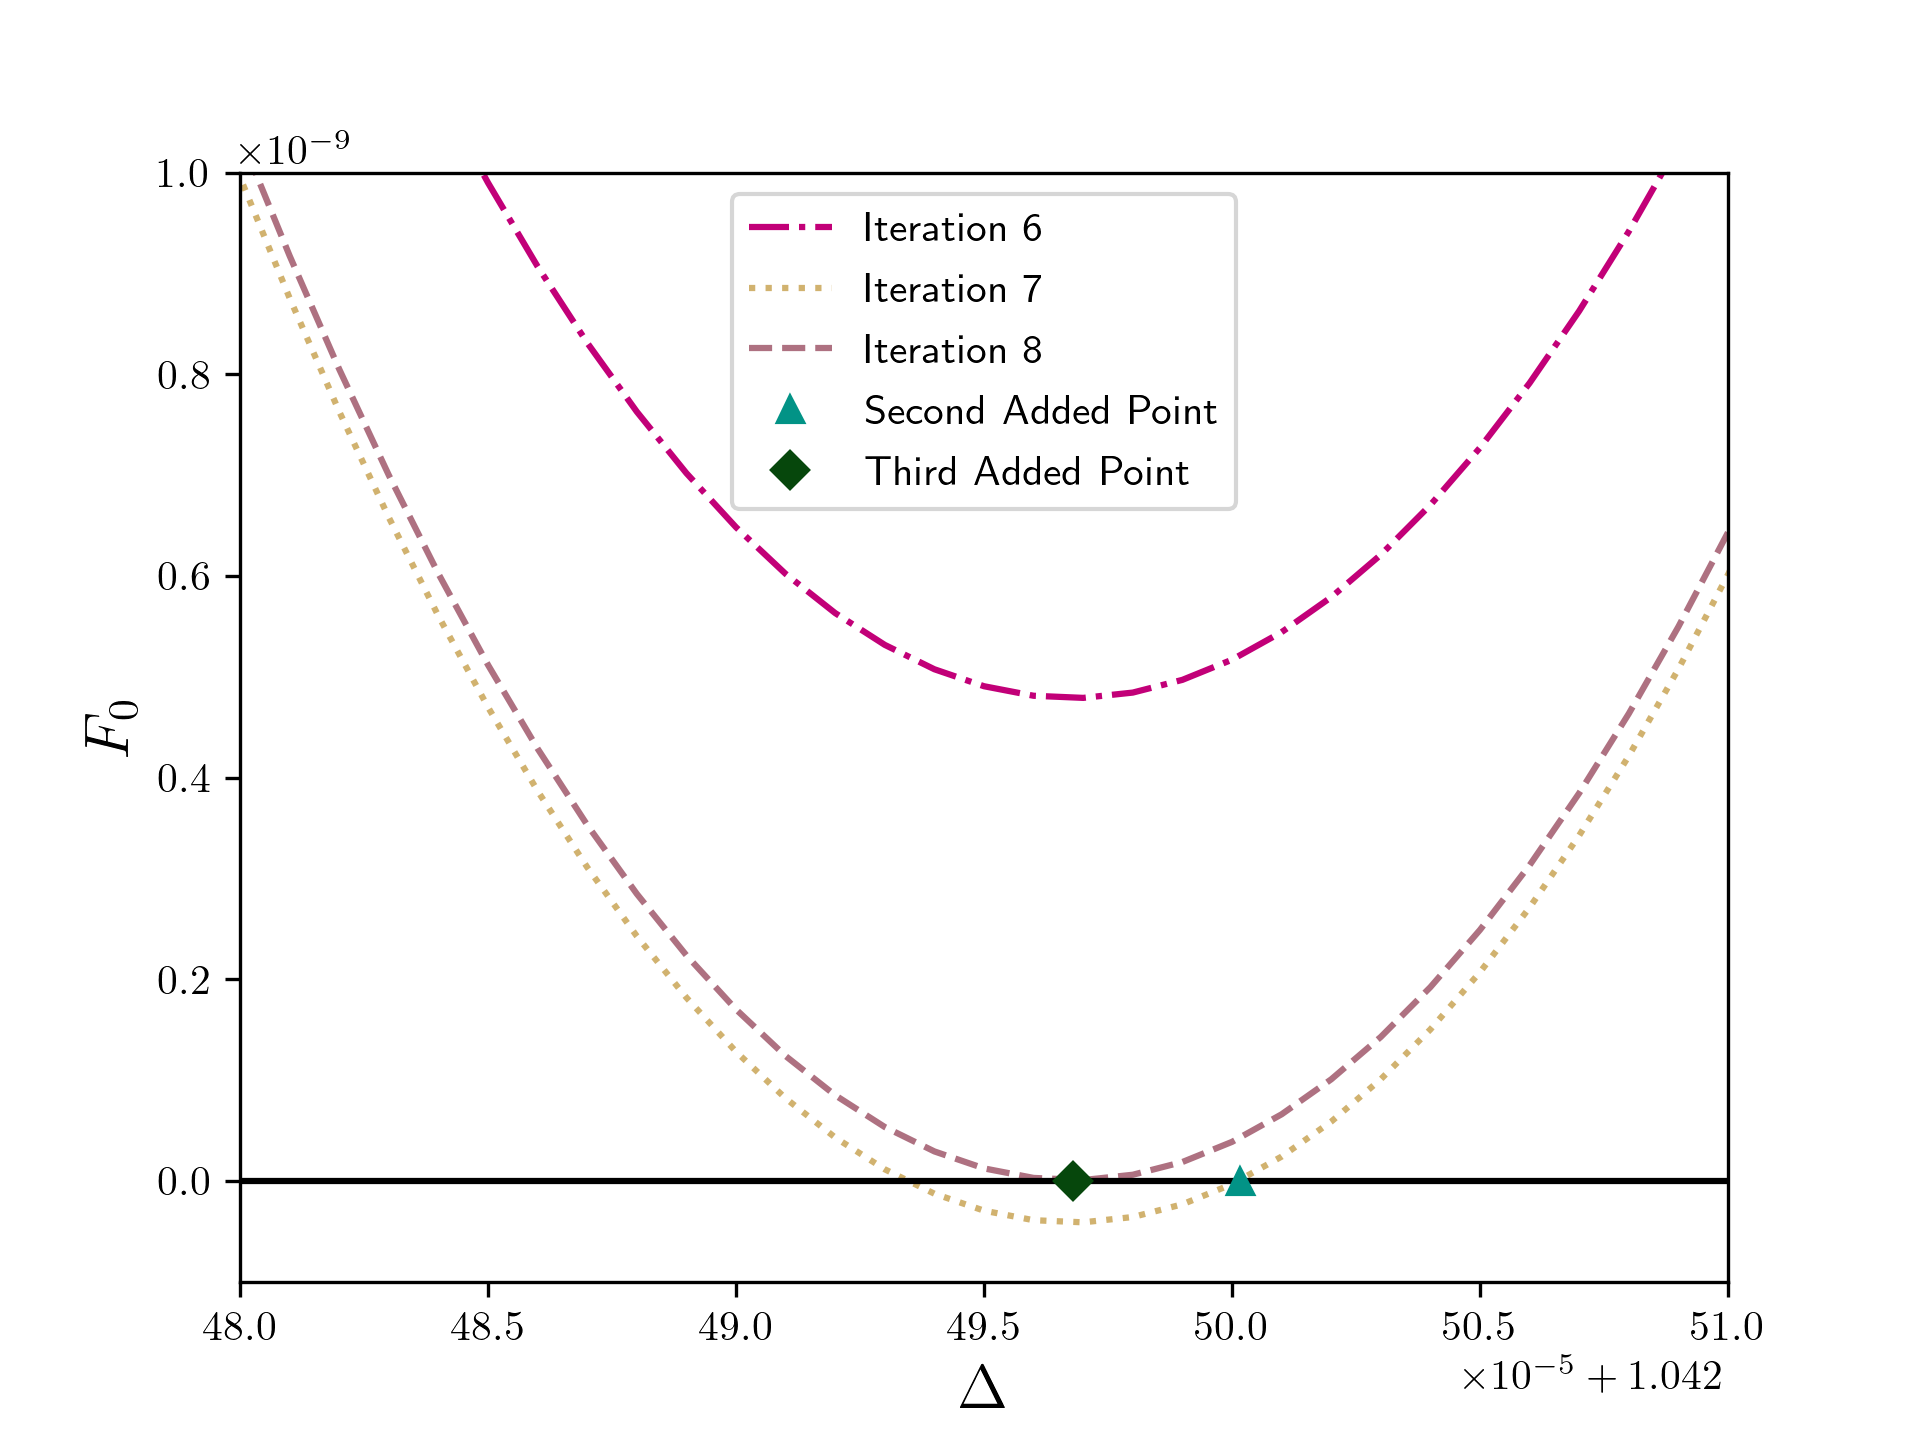
\includegraphics[width=0.9\textwidth]{outer_plots_3}
\end{center}
\caption{Plot of $F_{0}$ after the fifth, sixth, and seventh
  iterations, with duality gap thresholds of $1.05\times10^{-6}$,
  $1.02\times10^{-9}$, and $1.02\times10^{-9}$.  After the sixth
  iteration, \texttt{Outer\_Limits} adds a point at 1.042497.}
\label{fig:plot3}
\end{figure}

\pagebreak

\subsection{Termination}

\texttt{Outer\_Limits} can fail when the inner \texttt{SDPB} routines
fail, so \texttt{Outer\_Limits} has the same failure termination
criteria.  \texttt{Outer\_Limits}'s only successful termination
criteria is if the duality gap is less than
\texttt{dualityGapThreshold}.

\pagebreak

\subsection{Output File}

If \texttt{Outer\_Limits} completes successfully, it writes the
solution to a single JSON file, as shown in listing
\ref{listing:solution}.

\begin{lstlisting}[
  caption={Solution output of \texttt{Outer\_Limits} for the input file in listing~\ref{lst:points}},
  columns=fullflexible,
  label=listing:solution,
  keepspaces=true,
  basicstyle=\scriptsize\ttfamily\selectfont,
]
{
  "optimal": "1.840265763127732853472949500621348513754",
  "y":
  [
    "1",
    "-1.840265763127732853472949500621348513756"
  ],
  "options": 
{
    "maxIterations": "1000",
    "maxRuntime": "9223372036854775807",
    "checkpointInterval": "3600",
    "findPrimalFeasible": "false",
    "findDualFeasible": "false",
    "detectPrimalFeasibleJump": "false",
    "detectDualFeasibleJump": "false",
    "precision": "128",
    "precision_actual": "128",
    "dualityGapThreshold": "1e-10",
    "primalErrorThreshold": "1e-10",
    "dualErrorThreshold": "1e-10",
    "initialMatrixScalePrimal": "10",
    "initialMatrixScaleDual": "10",
    "feasibleCenteringParameter": "0.1",
    "infeasibleCenteringParameter": "0.3",
    "stepLengthReduction": "0.7",
    "maxComplementarity": "1e+100",
    "initialCheckpointDir": "test\/toy_functions.ck",
    "checkpointDir": "test\/toy_functions.ck",
    "functions": "test\/toy_functions.json",
    "points": "test\/toy_functions_points.json",
    "out": "test\/toy_functions_out.json",
    "dualityGapReduction": "1024",
    "writeSolution": "",
    "verbosity": "1"
}
}
\end{lstlisting}

\begin{thebibliography}{9}

\bibitem{DSD}
  David Simmons-Duffin,
  ``A Semidefinite Program Solver for the Conformal Bootstrap,"
  \href{http://arxiv.org/abs/1502.02033}{arXiv:1502.02033 [hep-th]}.

%\cite{Rychkov:2009ij}
\bibitem{Rychkov:2009ij} 
  V.~S.~Rychkov and A.~Vichi,
  ``Universal Constraints on Conformal Operator Dimensions,''
  Phys.\ Rev.\ D {\bf 80}, 045006 (2009)
  \href{http://arxiv.org/abs/0905.2211}{arXiv:0905.2211 [hep-th]}.
  %%CITATION = ARXIV:0905.2211;%%
  %82 citations counted in INSPIRE as of 05 Feb 2015

%\cite{Poland:2011ey}
\bibitem{Poland:2011ey} 
  D.~Poland, D.~Simmons-Duffin and A.~Vichi,
  ``Carving Out the Space of 4D CFTs,''
  JHEP {\bf 1205}, 110 (2012)
  \href{http://arXiv.org/abs/1109.5176}{arXiv:1109.5176 [hep-th]}.
  %%CITATION = ARXIV:1109.5176;%%
  %71 citations counted in INSPIRE as of 01 Feb 2015
  
%\cite{Kos:2013tga}
\bibitem{Kos:2013tga} 
  F.~Kos, D.~Poland and D.~Simmons-Duffin,
  ``Bootstrapping the $O(N)$ vector models,''
  JHEP {\bf 1406}, 091 (2014)
  \href{http://arXiv.org/abs/1307.6856}{arXiv:1307.6856 [hep-th]}.
  %%CITATION = ARXIV:1307.6856;%%
  %29 citations counted in INSPIRE as of 01 Feb 2015

%\cite{Kos:2014bka}
\bibitem{Kos:2014bka} 
  F.~Kos, D.~Poland and D.~Simmons-Duffin,
  ``Bootstrapping Mixed Correlators in the 3D Ising Model,''
  JHEP {\bf 1411}, 109 (2014)
  \href{http://arXiv.org/abs/1406.4858}{arXiv:1406.4858 [hep-th]}.
  %%CITATION = ARXIV:1406.4858;%%
  %9 citations counted in INSPIRE as of 01 Feb 2015

\bibitem{SDPA}
  M. Yamashita, K. Fujisawa, M. Fukuda, K. Nakata, and M. Nakata,
  ``A high-performance software package for semidefinite programs: SDPA 7,''
   Research Report B-463, Dept. of Mathematical and Computing Science, Tokyo Institute of Technology, Tokyo, Japan (2010).

\bibitem{SDPA2}
  M. Yamashita, K. Fujisawa, and M. Kojima,
  ``Implementation and evaluation of SDPA 6.0 (SemiDefinite Programming Algorithm 6.0),''
  Optimization Methods and Software" 18 491-505 (2003).

\bibitem{SDPAGMP}
  M. Nakata,
  ``A numerical evaluation of highly accurate multiple-precision arithmetic version of semidefinite programming solver: SDPA-GMP, -QD and -DD.,''
  2010 IEEE International Symposium on Computer-Aided Control System Design (CACSD), 29-34 Sept 2010.

\bibitem{BoostSite}
  C++ Standards Committee Library Working Group and other contributors,
  ``BOOST C++ Libraries,''
  \href{http://www.boost.org}{http://www.boost.org}.

\bibitem{libxml2}
  Gnome Project,
  Libxml2,
  \href{http://www.xmlsoft.org/}{http://www.xmlsoft.org/}

\bibitem{Elemental}
  J. Poulson, B. Marker, R. van de Geijn, J. Hammond, and N. Romero,
  ``Elemental: A new framework for distributed memory dense matrix computations, ACM Transactions on Mathematical Software,''
  ACM Trans. Math. Softw. 39 2 13:1-24 (2013),
  doi:10.1145/2427023.2427030
  
\bibitem{GMP}
  The GNU Multiprecision Library,
  \href{https://gmplib.org/}{https://gmplib.org/}

\bibitem{MPFR}
  The GNU MPFR Library,
  \href{https://www.mpfr.org/}{https://www.mpfr.org/}

\end{thebibliography}

\end{document}
